\pagebreak

\section{Simulation Results}
In this section, the simulation results are shown. Three simulations are run in total. The first simulation run is scaled by 50\% on the \textit{Dell Optiplex 9020} college computers. The second simulation run is scaled by 50\% on the \textit{university VMs}. The third simulation run is scaled by 90\% on \textit{university VMs}. Only the baseline of simulation 3 managed to reach 100\%. The list below is included in all scenarios of each simulation. The list provides an explanation of each statistic.

\begin{itemize}
    \setlength\itemsep{0em}
    \item Progress: The progress that the simulation made until it was terminated
    \item Time taken: The time the simulation ran for
    \item Events processed: The number of events processed
    \item Machine: The simulation machine
    \item Traffic Data: The date and time of the traffic data
    \item Parking Lot Data: The date and time of the parking lot data
    \item On-Street Initial Population: Initial population of on-street parking spaces
    \item Parking Duration Scale: Percentage indicating by how much parking space duration times are scaled down by
\end{itemize}

One of the evaluation metrics for this simulation is to compare the number of vehicles that had to re-route due to a parking space being taken. This evaluation metric is only outputted when simulations can reach 100\%.
Each simulation is set to run for 1800 simulation time, which equates to 30 minutes in real time.

\pagebreak

\subsection{Simulation run \#1}
In simulation \#1, all the relevant data is scaled by 50\%.
\subsubsection{Baseline}
\begin{itemize}
    \setlength\itemsep{0em}
    \item Progress: N/A\%
    \item Time taken: 2 days 18 hours
    \item Events processed: N/A
    \item Machine: Dell Optiplex 9020
    \item Traffic Data: 29\textsuperscript{th} April 2016 - 9:00am
    \item Parking Lot Data: 27\textsuperscript{th} February 2017 - 9:00am
    \item On-Street Initial Population: 95\% Occupied
    \item Parking Duration Scale: 50\%
\end{itemize}

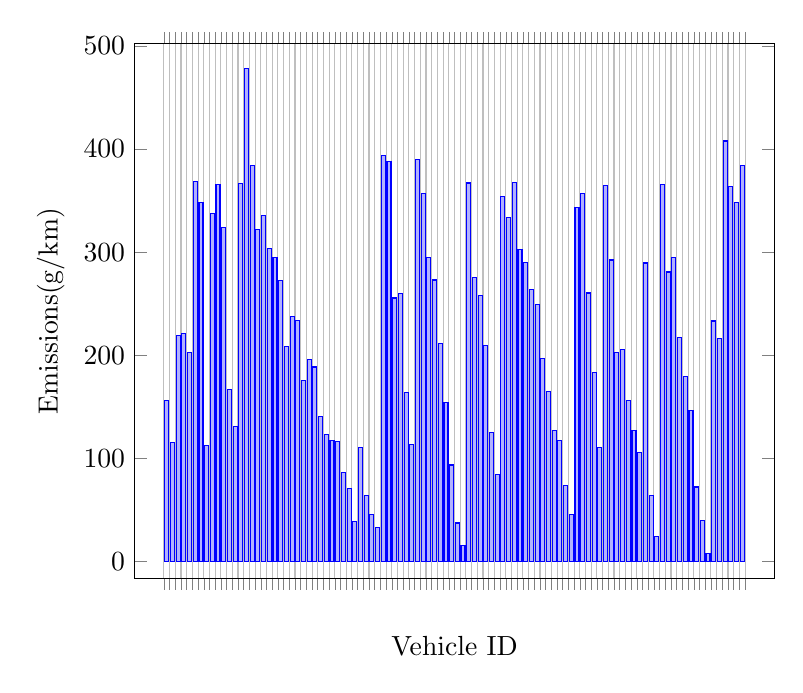
\begin{tikzpicture}
    \centering
        \begin{axis}[
                x tick label style={color=white},
                xlabel=Vehicle ID,
                ylabel=Emissions(g/km),
                enlargelimits=0.05,
                ybar interval=0.7,
                width=0.80\linewidth,
            ]
            \addplot 
                coordinates {(0,155.805159361) (1,115.658803469) (2,219.398923683) (3,220.973029414) (4,202.901627767) (5,368.526758022) (6,347.72994099) (7,112.858125185) (8,336.990266033) (9,365.379719613) (10,323.560140234) (11,166.742622625) (12,131.316792827) (13,366.555614167) (14,478.33034062) (15,384.192556648) (16,321.87890175) (17,335.392961233) (18,303.160461247) (19,294.82357699) (20,272.16886364) (21,208.469431409) (22,237.152775285) (23,233.346383293) (24,175.580418015) (25,195.453503171) (26,188.531566398) (27,140.666140823) (28,122.736776705) (29,117.110654483) (30,116.337779579) (31,86.2587981483) (32,70.3461742587) (33,38.8751431569) (34,110.941216363) (35,64.2100598048) (36,45.9631080107) (37,33.328077527) (38,393.962110852) (39,387.604415516) (40,255.500165751) (41,259.854598833) (42,164.176319463) (43,113.133708908) (44,389.480164573) (45,356.840680174) (46,294.488060139) (47,272.936508712) (48,210.933089822) (49,154.235578191) (50,93.5543151606) (51,37.299671071) (52,15.2660962934) (53,366.993296469) (54,275.640936132) (55,257.959744226) (56,209.786097832) (57,124.834702615) (58,84.5390519345) (59,354.287203996) (60,333.525756683) (61,367.224427932) (62,302.201551134) (63,289.762782158) (64,263.80044816) (65,248.931742846) (66,196.825338488) (67,164.692800677) (68,127.025483251) (69,116.917349523) (70,73.7810961086) (71,45.8458459587) (72,343.49111192) (73,356.6459616) (74,260.350875888) (75,183.4538446) (76,110.573466909) (77,364.210095816) (78,292.305263466) (79,202.726352587) (80,205.469930278) (81,156.510247308) (82,127.22297677) (83,105.965419289) (84,289.372461959) (85,64.005270681) (86,24.054127114) (87,365.714043759) (88,280.661318998) (89,294.591705863) (90,217.587431534) (91,179.624030697) (92,145.977738451) (93,72.2270265008) (94,39.6657934931) (95,7.42066276002) (96,233.210742148) (97,216.281837583) (98,407.721609014) (99,363.327616872) (100,348.24325321) (101,383.96692404) (102,271.226320406)};
        \end{axis}
\end{tikzpicture}

Average Emissions: 218.711648476g/km

\pagebreak

\subsubsection{VANET}
\begin{itemize}
    \setlength\itemsep{0em}
    \item Progress: N/A\%
    \item Time taken:  3 days 15 hours
    \item Events processed: N/A
    \item Machine: Dell Optiplex 9020
    \item Traffic Data: 29\textsuperscript{th} April 2016 - 9:00am
    \item Parking Lot Data: 27\textsuperscript{th} February 2017 - 9:00am
    \item On-Street Initial Population: 95\% Occupied
    \item Parking Duration Scale: 50\%
\end{itemize}

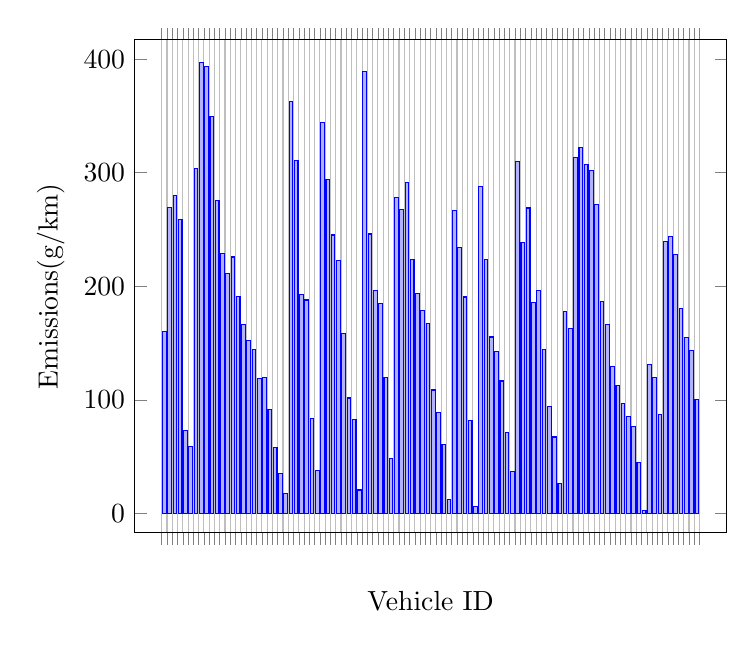
\begin{tikzpicture}
    \centering
        \begin{axis}[
                x tick label style={color=white},
                xlabel=Vehicle ID,
                ylabel=Emissions(g/km),
                enlargelimits=0.05,
                ybar interval=0.7,
                width=0.75\linewidth,
            ]
            \addplot 
                coordinates {(0,160.3335638793) (1,269.1147059284) (2,280.02684511864) (3,259.15322707701) (4,73.323917014134) (5,59.266105470196) (6,303.5476783495) (7,397.34711079019) (8,393.30207405967) (9,349.87354132696) (10,275.204895426) (11,228.86750515556) (12,210.97108663498) (13,225.83876263129) (14,190.71444439368) (15,166.16920196126) (16,152.63309647394) (17,144.14725916212) (18,118.74398042956) (19,119.61125874272) (20,91.442373854083) (21,58.083474959498) (22,35.276450163302) (23,17.866053011013) (24,362.57044756664) (25,311.16132970467) (26,192.86780069856) (27,187.99445375043) (28,83.977807058915) (29,38.004046720472) (30,344.33145078467) (31,293.8444882838) (32,245.18531533967) (33,222.82212268939) (34,158.46231452176) (35,101.70636614091) (36,82.665597567671) (37,20.648513084336) (38,389.06508552456) (39,246.04711130284) (40,196.03183557977) (41,184.55611056815) (42,119.94980920157) (43,48.296047599982) (44,278.0970015235) (45,267.36696594356) (46,291.27072970019) (47,223.4654211581) (48,193.62363433212) (49,178.73425174337) (50,167.03405039366) (51,108.7145511002) (52,89.265741280142) (53,61.04620157541) (54,12.596723422571) (55,266.50291150454) (56,234.04470060659) (57,190.57504385732) (58,81.594013340399) (59,5.9190685695805) (60,288.1669366819) (61,223.62400033473) (62,155.40399375807) (63,142.77964231562) (64,116.59245244349) (65,71.32333027314) (66,36.822944292686) (67,309.8967197539) (68,238.81477235454) (69,268.96481935571) (70,185.747721905) (71,196.52452486113) (72,144.34476732611) (73,93.845008867101) (74,67.345421431236) (75,26.468095176686) (76,178.07131753452) (77,162.54118833328) (78,313.60082787459) (79,322.50159281904) (80,307.42276046791) (81,301.88312328778) (82,272.3714659275) (83,186.31686936026) (84,166.733991435) (85,129.01838512718) (86,112.75918867032) (87,96.897424574197) (88,85.674538079603) (89,76.606814234189) (90,45.066874781376) (91,2.6791459209701) (92,131.38021262772) (93,119.88434840369) (94,86.784813294427) (95,239.55885830629) (96,243.63976855396) (97,228.27846020777) (98,180.40693847647) (99,154.97871109087) (100,143.81736804371) (101,100.10783440313) (102,48.590652533668)};
        \end{axis}
\end{tikzpicture}

Average Emissions: 175.389672828g/km

\subsubsection{Conclusion}
Both graphs of simulation \#1 show the first 103 vehicles that entered their corresponding simulation. Within the first 103 vehicles range, the \ac{VANET} model resulted in fewer emissions. However, neither simulations were able to finish. Thus the results are not comparable.

\pagebreak

\subsection{Simulation run \#2}
In simulation \#2, all the relevant data is scaled by 50\%. 
\subsubsection{Baseline}
\begin{itemize}
    \setlength\itemsep{0em}
    \item Progress: 53\%
    \item Time taken: 9 days 12 hours
    \item Events processed: \texttildelow 400 million
    \item Machine: University VM
    \item Traffic Data: 29\textsuperscript{th} April 2016 - 9:00am
    \item Parking Lot Data: 27\textsuperscript{th} February 2017 - 9:00am
    \item On-Street Initial Population: 95\% Occupied
    \item Parking Duration Scale: 50\%
\end{itemize}

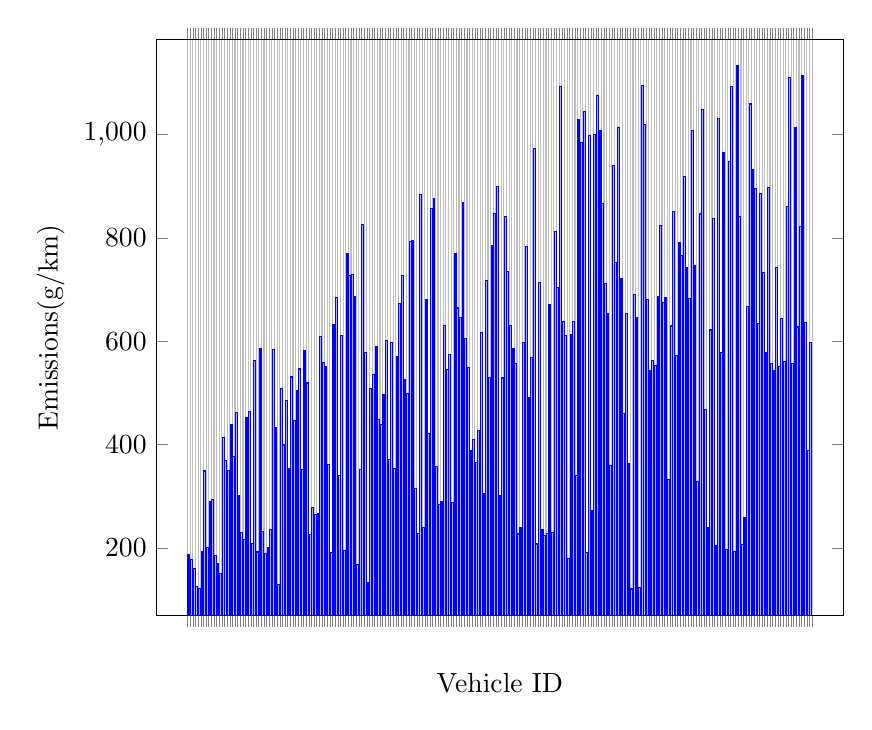
\begin{tikzpicture}
    \centering
        \begin{axis}[
                x tick label style={color=white},
                xlabel=Vehicle ID,
                ylabel=Emissions(g/km),
                enlargelimits=0.05,
                ybar interval=0.7,
                width=0.85\linewidth,
            ]
            \addplot 
                coordinates {(0,187.47097560966) (1,177.76292715954) (2,160.82470417734) (3,124.59476867463) (4,120.96565825213) (5,193.50824041774) (6,348.71206683708) (7,201.46078758648) (8,289.13193284549) (9,293.24709198077) (10,184.96517915762) (11,170.04380617893) (12,150.14706797266) (13,413.28049361898) (14,369.0938398479) (15,350.09767450918) (16,438.7246780865) (17,376.83210395823) (18,462.1070237032) (19,300.49784900916) (20,229.16455006373) (21,215.29669107783) (22,451.61914408946) (23,463.78531109125) (24,208.24720803206) (25,563.15454812896) (26,191.96015919823) (27,586.21786111848) (28,231.92361327969) (29,189.5425560569) (30,200.97640786842) (31,236.15101644463) (32,583.32493580091) (33,432.8895470674) (34,129.78516398554) (35,507.66452627022) (36,399.09483292712) (37,485.81292868297) (38,353.9647223179) (39,530.73069858335) (40,446.72419658488) (41,503.6715207291) (42,546.29598552113) (43,352.2738418505) (44,581.16360605745) (45,519.00050726117) (46,225.45651778201) (47,277.59707569242) (48,265.08896775265) (49,265.75760467268) (50,609.1586097341) (51,558.62646822942) (52,551.41943411942) (53,361.80847723384) (54,191.24730104598) (55,632.4462834619) (56,684.97450624477) (57,340.55612252445) (58,611.37567635826) (59,195.63685832662) (60,769.59911247457) (61,727.31860415182) (62,729.13710714931) (63,685.58761844639) (64,167.06358434058) (65,352.23893278568) (66,825.38056194509) (67,577.9012138503) (68,132.14542402769) (69,507.67285503615) (70,536.17776444681) (71,590.5836220391) (72,448.08357547522) (73,438.69925693151) (74,495.87879205697) (75,600.84366620726) (76,370.84028578032) (77,597.18495532663) (78,354.08012568901) (79,570.15031083608) (80,672.64836491031) (81,726.57945976419) (82,525.06714611366) (83,498.06420995689) (84,792.31632908383) (85,795.19521713675) (86,315.68015108507) (87,227.44094685137) (88,884.68733117806) (89,239.78324510086) (90,680.44445390714) (91,421.95105149867) (92,856.97207277293) (93,876.39374168065) (94,356.84358309867) (95,284.426185545) (96,289.31328796759) (97,631.14755816245) (98,545.63465803456) (99,573.52553348842) (100,287.21613684582) (101,769.5045415967) (102,664.21165924622) (103,645.61469982141) (104,868.62841485164) (105,605.42920028674) (106,548.39709980201) (107,389.23005343843) (108,410.13418324115) (109,365.03296366356) (110,427.58767065676) (111,617.67434279942) (112,304.24625948015) (113,717.10139583154) (114,530.42569951093) (115,785.06104604947) (116,847.19233495332) (117,899.53714104323) (118,300.55918947999) (119,528.78769404177) (120,841.81718283527) (121,734.52670244313) (122,630.41378093843) (123,584.82393812653) (124,557.66269348928) (125,226.75419295658) (126,238.44004958261) (127,597.01531452465) (128,784.07939911072) (129,490.04941818639) (130,568.09196253444) (131,973.59958090724) (132,207.35925159673) (133,713.92372534891) (134,236.09788796684) (135,223.1197557738) (136,226.89853140832) (137,670.61735740498) (138,230.2042419875) (139,811.8100930135) (140,704.16070852287) (141,1092.2590761246) (142,638.55489932815) (143,610.80535960726) (144,180.07180065674) (145,612.64795697225) (146,637.67923402161) (147,340.67007021472) (148,1029.0084240539) (149,985.34436349067) (150,1044.6422220544) (151,191.10065457238) (152,997.86039878203) (153,272.08496906811) (154,999.52205655198) (155,1075.7660976945) (156,1007.7968815161) (157,867.01039177596) (158,711.682505057) (159,652.98548925173) (160,359.3720612273) (161,940.00239513204) (162,752.0863470292) (163,1013.4563388568) (164,720.33627846405) (165,459.86553906798) (166,654.36147260833) (167,363.56554917781) (168,120.22635005919) (169,690.13907841861) (170,646.38547134942) (171,123.30485451717) (172,1094.4609779693) (173,1019.3112710277) (174,680.54233766262) (175,544.0720663861) (176,562.21029659734) (177,553.4131030779) (178,686.00753729256) (179,824.08586446878) (180,674.73515874624) (181,684.44218005821) (182,332.38543788871) (183,629.36465993602) (184,851.67400638704) (185,572.22625544875) (186,790.20942067252) (187,765.67400414286) (188,918.40812335239) (189,741.75027340495) (190,681.92659899162) (191,1008.5198300536) (192,746.37615477158) (193,329.16334745607) (194,846.31200364407) (195,1047.708038566) (196,467.18195980361) (197,238.29592992404) (198,621.72136385627) (199,837.86702389626) (200,204.2509425175) (201,1031.900185186) (202,577.43637135745) (203,965.27951078905) (204,196.24253430473) (205,948.42962474697) (206,1093.9171403127) (207,193.56087823303) (208,1132.9411602975) (209,840.65297370206) (210,206.08862949471) (211,259.26388815972) (212,667.00558949313) (213,1059.1623656077) (214,931.4291151615) (215,896.44234537227) (216,635.02254599399) (217,886.00403996751) (218,732.38015259726) (219,577.86336779962) (220,898.40434846215) (221,557.60967896322) (222,544.14671635914) (223,742.79759601687) (224,550.57232836393) (225,644.05224744772) (226,561.56938298163) (227,860.70827660299) (228,1109.9232719363) (229,556.04661520039) (230,1014.3757748555) (231,627.52175013822) (232,821.99450140863) (233,1114.3863984734) (234,636.02870443992) (235,388.84099144749) (236,597.48074768776) (237,1104.1263841698)};
        \end{axis}
\end{tikzpicture}

Average Emissions: 561.198626609g/km

\pagebreak

\subsubsection{VANET}
\begin{itemize}
    \setlength\itemsep{0em}
    \item Progress: 10\%
    \item Time taken: 4 days 9 hours
    \item Events processed: \texttildelow 17 million
    \item Machine: University VM
    \item Traffic Data: 29\textsuperscript{th} April 2016 - 9:00am
    \item Parking Lot Data: 27\textsuperscript{th} February 2017 - 9:00am
    \item On-Street Initial Population: 95\% Occupied
    \item Parking Duration Scale: 50\%
\end{itemize}

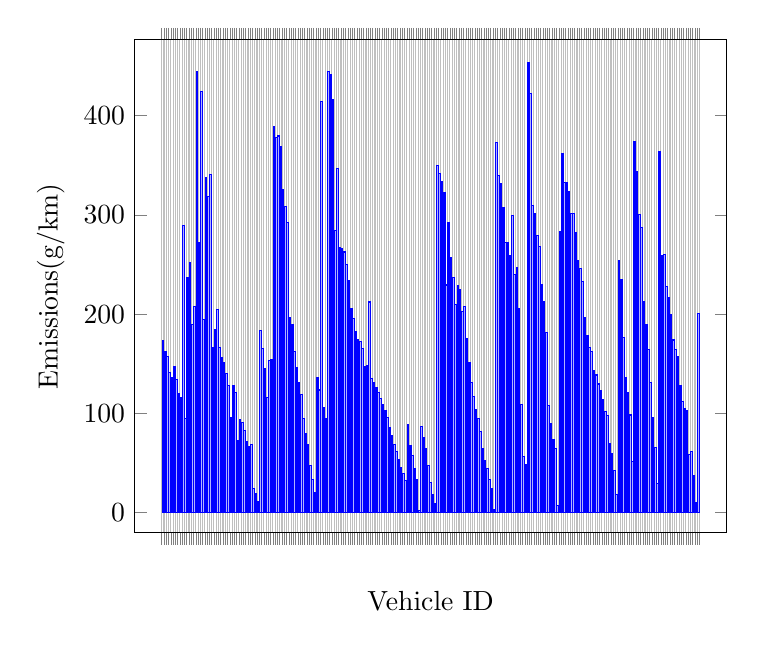
\begin{tikzpicture}
    \centering
        \begin{axis}[
                x tick label style={color=white},
                xlabel=Vehicle ID,
                ylabel=Emissions(g/km),
                enlargelimits=0.05,
                ybar interval=0.7,
                width=0.75\linewidth,
            ]
            \addplot 
                coordinates {(0, 173.26418876382) (1, 162.62268386015) (2, 157.64549294729) (3, 140.99612792042) (4, 135.93284744986) (5, 146.90075514854) (6, 134.1995749369) (7, 119.99992709463) (8, 116.36632163992) (9, 289.43388617448) (10, 95.309858744281) (11, 237.38602530863) (12, 252.17046638946) (13, 189.37174026117) (14, 207.33007121591) (15, 444.28387838163) (16, 271.97890125564) (17, 424.23542621343) (18, 194.8547697935) (19, 337.97468836358) (20, 318.64580673625) (21, 341.1057024257) (22, 166.68008437825) (23, 184.02547895553) (24, 204.71281668502) (25, 166.66900949246) (26, 156.63733893478) (27, 151.73447716469) (28, 140.33777724039) (29, 128.04673252073) (30, 96.121171692893) (31, 127.97814011918) (32, 120.72733818248) (33, 72.974597916125) (34, 93.601798401605) (35, 91.297706271659) (36, 82.705564622246) (37, 71.533578670891) (38, 66.678686802015) (39, 68.477950684323) (40, 23.994006900634) (41, 19.103782090286) (42, 10.858276989634) (43, 183.71990296228) (44, 165.00430588617) (45, 145.00251591869) (46, 115.67239931677) (47, 153.36955962072) (48, 153.96359391121) (49, 389.34833004043) (50, 378.32850137194) (51, 379.51811218916) (52, 369.22893059749) (53, 325.20375237382) (54, 308.09771334225) (55, 292.66540126774) (56, 196.47350004986) (57, 189.40091479072) (58, 162.73926351943) (59, 146.09171571418) (60, 131.22876975946) (61, 118.6796846161) (62, 94.785276064116) (63, 80.036680520143) (64, 68.515502707105) (65, 47.408738586773) (66, 33.176227245148) (67, 20.28596492566) (68, 136.637314232) (69, 123.63563999546) (70, 414.36213872165) (71, 106.01632325086) (72, 95.250687851703) (73, 444.11018593429) (74, 441.85073043916) (75, 416.39583491492) (76, 283.89633586428) (77, 346.85305782009) (78, 267.3249568759) (79, 265.79036446502) (80, 262.67458168749) (81, 249.93187557418) (82, 234.25692285618) (83, 205.58217628011) (84, 195.33929306836) (85, 182.76060124631) (86, 174.05417698365) (87, 172.08412529054) (88, 164.99848711689) (89, 147.15702959038) (90, 147.94455254053) (91, 212.31037653001) (92, 134.78832867237) (93, 130.8980899727) (94, 126.15129324539) (95, 120.78455997091) (96, 114.89544067784) (97, 108.79166856479) (98, 103.11051120854) (99, 95.846523251839) (100, 85.451815114686) (101, 77.559707507178) (102, 68.835389116702) (103, 61.304061324118) (104, 53.890340156895) (105, 45.76231322176) (106, 39.734224554843) (107, 32.432165566037) (108, 89.189948684741) (109, 67.70758474593) (110, 57.315288103028) (111, 44.457785769271) (112, 33.834254184138) (113, 2.2643980051185) (114, 86.71580710946) (115, 75.242112417808) (116, 64.937416493286) (117, 47.272859675245) (118, 30.124892636294) (119, 18.602808742986) (120, 9.2665944106122) (121, 349.74803276755) (122, 341.6270206664) (123, 333.25662691009) (124, 322.96216004076) (125, 229.43664153834) (126, 292.33657136267) (127, 257.4865527359) (128, 237.39859203556) (129, 209.63616735486) (130, 229.34420311479) (131, 224.79913393485) (132, 203.09377725396) (133, 207.38897133566) (134, 175.63893098147) (135, 151.42770560773) (136, 131.14277392014) (137, 117.33692736581) (138, 104.2978989815) (139, 95.014552964337) (140, 82.093404381793) (141, 64.423128970813) (142, 52.508257434475) (143, 44.807859910994) (144, 33.195328855746) (145, 24.341060631746) (146, 3.1757392814795) (147, 373.13488593904) (148, 339.94202479333) (149, 331.85961223189) (150, 307.82379234965) (151, 272.29907776751) (152, 272.65572379594) (153, 259.49395179068) (154, 299.46670783363) (155, 239.74383516549) (156, 247.16171047142) (157, 205.64216592894) (158, 109.41220473028) (159, 56.311081794032) (160, 48.045996597522) (161, 453.92123647372) (162, 422.08250697556) (163, 309.80285540327) (164, 301.70913450598) (165, 279.1405672606) (166, 268.13153905031) (167, 229.37039709991) (168, 212.64342194618) (169, 181.92026018596) (170, 107.7895283836) (171, 89.451884361576) (172, 73.706837604886) (173, 64.484172887062) (174, 7.5618556638862) (175, 283.6381796035) (176, 362.0901497133) (177, 332.77105871091) (178, 332.64525675332) (179, 323.26247892528) (180, 301.2166269904) (181, 301.11353944374) (182, 282.2239155006) (183, 253.99638976852) (184, 245.68791194042) (185, 232.73020590978) (186, 196.78479915725) (187, 178.03003372102) (188, 166.35593669292) (189, 162.72917396914) (190, 142.85361810066) (191, 138.68481810856) (192, 129.62839848027) (193, 122.66544803362) (194, 113.56099192458) (195, 102.11752934395) (196, 97.575495996907) (197, 70.047894720225) (198, 59.952963023982) (199, 42.56608486313) (200, 17.989635780979) (201, 254.43790186105) (202, 235.25576909297) (203, 176.76849982163) (204, 136.553021979) (205, 120.74048124424) (206, 98.468481969518) (207, 51.644892175653) (208, 374.41352201215) (209, 343.34783313894) (210, 300.2321212131) (211, 287.06083124693) (212, 212.39467844221) (213, 189.62081758173) (214, 164.11513481785) (215, 131.10990804578) (216, 96.028597441333) (217, 65.393333718371) (218, 29.751549121158) (219, 363.46791793513) (220, 259.11673396971) (221, 259.77604804412) (222, 227.8604119258) (223, 216.53099127244) (224, 199.41707009544) (225, 173.96171295745) (226, 163.97619241655) (227, 157.38056606059) (228, 127.84223519108) (229, 112.41783053062) (230, 105.24997852559) (231, 102.87780779067) (232, 58.525247994491) (233, 61.289407945651) (234, 37.736104000377) (235, 10.501524326879) (236, 200.83921112804) (237, 200.79088804853)};
        \end{axis}
\end{tikzpicture}

Average Emissions: 175.149905231g/km

\subsubsection{Conclusion}
The gap between baseline and \ac{VANET} models in simulation run \#two are incomparable. The process took too long, and a decision was made to terminate the simulations. The simulation is then re-scaled and repeated for simulation \#3.

\pagebreak

\subsection{Simulation run \#3}
In simulation \#3, all the relevant data is scaled by 90\%

\subsubsection{Baseline}
\begin{itemize}
    \setlength\itemsep{0em}
    \item Progress: 100\%
    \item Time taken: 1d 10hr
    \item Events processed: \texttildelow 7 million
    \item Machine: University VM
    \item Traffic Data: 29\textsuperscript{th} April 2016 - 9:00am
    \item Parking Lot Data: 27\textsuperscript{th} February 2017 - 9:00am
    \item On-Street Initial Population: 95\% Occupied
    \item Parking Duration Scale: 90\%
\end{itemize}

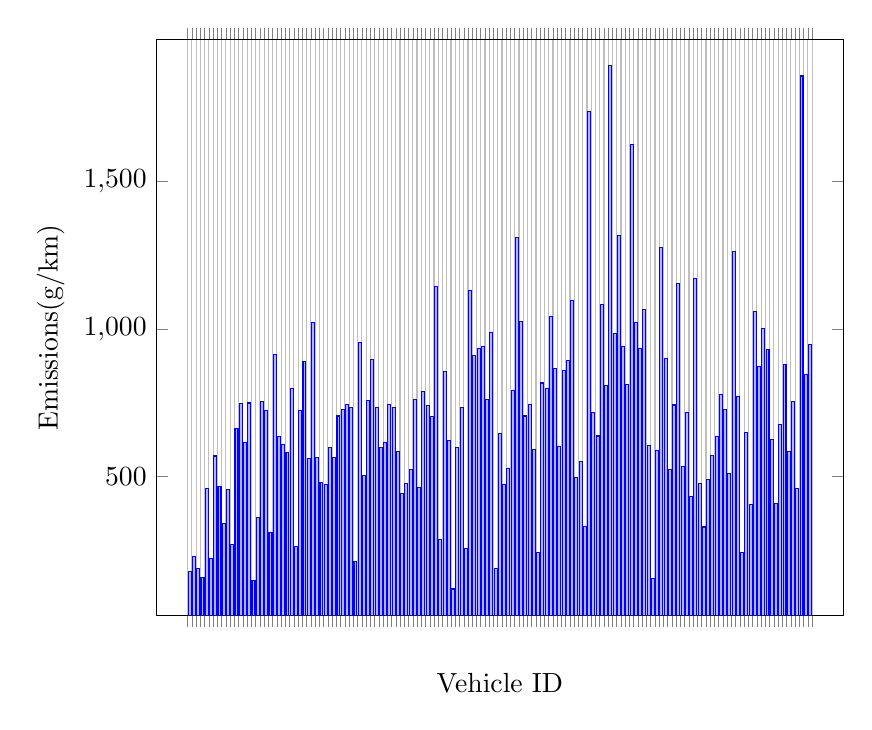
\begin{tikzpicture}
    \centering
        \begin{axis}[
                x tick label style={color=white},
                xlabel=Vehicle ID,
                ylabel=Emissions(g/km),
                enlargelimits=0.05,
                ybar interval=0.7,
                width=0.85\linewidth,
            ]
            \addplot 
                coordinates { (0,177.34212018003) (1,228.35539591857) (2,187.66737670924) (3,155.94824347081) (4,459.21267806871) (5,220.47425513642) (6,569.06190147975) (7,466.52144287313) (8,341.70684424958) (9,456.44397824916) (10,269.88944183195) (11,661.76214320568) (12,746.2480891099) (13,616.0350755922) (14,748.58577596478) (15,148.20272294781) (16,362.04299856637) (17,752.70066434657) (18,722.19856219695) (19,309.94845029992) (20,911.99664829129) (21,634.80310629941) (22,607.42344353307) (23,581.97648096876) (24,798.74707236171) (25,263.44258646751) (26,721.66655984159) (27,889.55889693331) (28,560.40129415186) (29,1021.6242348576) (30,564.2519507985) (31,480.41406233828) (32,471.95725760051) (33,596.55261545801) (34,563.50080166717) (35,704.50005254038) (36,726.82783485835) (37,744.29310834345) (38,733.50985734184) (39,212.18494002036) (40,953.54887237154) (41,502.98608896446) (42,757.56517954389) (43,896.1627220036) (44,734.77725966551) (45,597.69158664543) (46,613.91137016586) (47,744.21163803969) (48,734.24825282685) (49,584.70832132475) (50,441.87376166593) (51,475.92350145778) (52,523.49041601975) (53,759.40064065534) (54,461.74864368009) (55,786.50532070193) (56,741.12191695914) (57,702.81108648302) (58,1143.8913104419) (59,285.3610765187) (60,854.52632374121) (61,621.66803478486) (62,118.07246044372) (63,597.71652361896) (64,733.6660517959) (65,253.98250233626) (66,1130.6599854391) (67,910.29984927835) (68,932.85907368651) (69,939.72667602974) (70,761.16252863561) (71,988.0534120996) (72,187.1952579455) (73,643.85072626462) (74,471.3583447065) (75,526.28056551198) (76,792.02971712246) (77,1309.6693909989) (78,1023.7280621448) (79,704.36764556736) (80,743.11010718274) (81,589.55972537108) (82,240.88876247989) (83,816.33308723757) (84,799.10547652068) (85,1042.0431542294) (86,866.08726867163) (87,601.53087350658) (88,860.19309348325) (89,892.7326782481) (90,1095.1350388104) (91,496.84034504181) (92,549.460484654) (93,329.66017080886) (94,1735.7376381639) (95,717.70313905578) (96,636.69215461312) (97,1081.9879567746) (98,807.42864264938) (99,1891.0321515973) (100,983.87496036361) (101,1316.0876082402) (102,940.97125498591) (103,811.01341890482) (104,1626.0841902303) (105,1021.7902334014) (106,934.03093284648) (107,1064.2181728818) (108,605.33673242565) (109,154.13405837146) (110,586.14368868359) (111,1277.0737221512) (112,900.66414274129) (113,523.34862239829) (114,741.70887207972) (115,1152.8513920462) (116,534.69470352447) (117,716.78384371387) (118,433.06246348729) (119,1169.1813233604) (120,475.07781101176) (121,328.23141404929) (122,489.07481794988) (123,571.75866356795) (124,633.55333700404) (125,776.3540265469) (126,727.3549333114) (127,509.72819913516) (128,1260.8762574435) (129,771.88319985076) (130,241.8058380791) (131,648.52752981514) (132,404.30776455866) (133,1057.4164144849) (134,872.81935108825) (135,1001.7101155797) (136,929.19879530347) (137,625.09377640873) (138,408.46128043457) (139,676.2388255074) (140,878.01616236398) (141,585.35071374297) (142,753.38965120442) (143,459.01694405407) (144,1856.9411265604) (145,844.06882372673) (146,946.85800903538) (147,836.42962773428)};
        \end{axis}
\end{tikzpicture}

Average Emissions: 703.977383507g/km \\
\indent Number of vehicles that had to re-route: 76 vehicles

\pagebreak

\subsubsection{VANET}
\begin{itemize}
    \setlength\itemsep{0em}
    \item Progress: 100\%
    \item Time taken: 1d 6hr
    \item Events processed: \texttildelow 10 million
    \item Machine: University VM
    \item Traffic Data: 29\textsuperscript{th} April 2016 - 9:00am
    \item Parking Lot Data: 27\textsuperscript{th} February 2017 - 9:00am
    \item On-Street Initial Population: 95\% Occupied
    \item Parking Duration Scale: 90\%
\end{itemize}

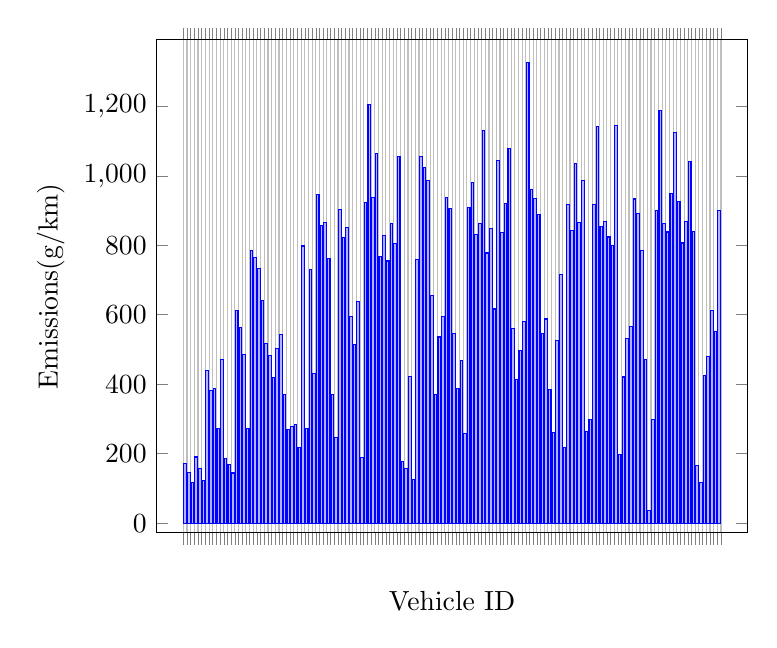
\begin{tikzpicture}
    \centering
        \begin{axis}[
                x tick label style={color=white},
                xlabel=Vehicle ID,
                ylabel=Emissions(g/km),
                enlargelimits=0.05,
                ybar interval=0.7,
                width=0.75\linewidth,
            ]
            \addplot 
                coordinates {(0,171.08795762172) (1,146.44388881286) (2,117.10977702573) (3,190.29385206117) (4,157.78831685736) (5,123.19350138837) (6,440.18207886707) (7,381.95892749404) (8,388.76910707504) (9,273.14928311298) (10,471.71461211813) (11,185.42929856546) (12,169.53172298444) (13,144.44353656057) (14,612.60778938777) (15,563.0235426444) (16,484.50748694151) (17,271.81354937215) (18,784.4780767906) (19,763.88778504603) (20,732.59146149393) (21,641.21403029295) (22,517.41472798648) (23,483.37489438616) (24,419.36021583265) (25,503.44532571024) (26,542.22793084913) (27,371.24865042591) (28,270.44959219927) (29,277.47987314593) (30,284.1704444155) (31,217.56154716472) (32,797.87351646974) (33,271.24049287005) (34,731.02108742825) (35,430.870389488) (36,946.70759465043) (37,857.61531084135) (38,865.34695475889) (39,762.33188181687) (40,370.53541187282) (41,247.01161032016) (42,904.35359201607) (43,822.3567225978) (44,852.32091311494) (45,594.97774452224) (46,514.03120873979) (47,638.46080073533) (48,188.39244609416) (49,923.18077850145) (50,1204.5121499643) (51,938.70416894142) (52,1065.1930823024) (53,767.89255136865) (54,828.0167474981) (55,754.80687771544) (56,863.27318281506) (57,805.4527510349) (58,1055.5985979283) (59,176.25009339392) (60,156.90667265334) (61,422.26523536965) (62,124.30664825145) (63,758.47713837078) (64,1054.6593512578) (65,1025.2546493127) (66,986.58493122264) (67,654.54429108507) (68,370.34023690352) (69,535.80359964526) (70,595.22633220252) (71,938.85109546852) (72,906.30782836102) (73,546.65855160861) (74,386.8248377151) (75,467.16780170572) (76,257.34076301063) (77,908.20872165253) (78,980.89949072302) (79,830.62900143735) (80,863.50149063243) (81,1129.4763831846) (82,777.72377510138) (83,848.53359406346) (84,616.67087515038) (85,1044.3417156753) (86,837.75006866387) (87,920.24351821204) (88,1078.9181196292) (89,561.35183158076) (90,413.82774056066) (91,497.70846270387) (92,581.17771686723) (93,1327.3354562684) (94,960.28954912124) (95,935.02563412353) (96,887.53070902377) (97,546.54308774642) (98,587.86665845206) (99,384.30175274087) (100,261.36990201402) (101,527.08763209699) (102,716.86928991137) (103,216.91936029873) (104,917.27758684561) (105,842.8946592558) (106,1036.2954366832) (107,865.65801112031) (108,985.4809928628) (109,264.32509071198) (110,299.01308315142) (111,916.64934078444) (112,1142.3786218597) (113,853.73119567271) (114,868.0054969663) (115,823.89930808487) (116,799.0204194202) (117,1144.3139569005) (118,197.82518142479) (119,420.85786369057) (120,531.19612748524) (121,567.41496242988) (122,933.23114066646) (123,890.6579118404) (124,785.31049470536) (125,470.68781348384) (126,36.519235721848) (127,298.03195215971) (128,899.75428260339) (129,1188.0520780228) (130,862.2615927713) (131,838.42050865036) (132,949.86628691073) (133,1126.0546162701) (134,925.90584489222) (135,806.71141321828) (136,867.27509256526) (137,1040.1183525855) (138,839.77242265654) (139,164.66653746299) (140,117.2799922961) (141,425.76973142692) (142,480.89136351664) (143,611.56125715681) (144,551.33418208965) (145,901.47171212059) (146,864.78185842514) };
        \end{axis}
\end{tikzpicture}

Average Emissions: 639.881142556g/km \\
\indent Number of vehicle that had to re-route: 64 vehicles

\subsubsection{Conclusion}
The results show the 146 vehicles, with their completed time through the simulation. The average emissions produced in the \ac{VANET} model is observed to be less than that of the baseline model. As well as this, the number of vehicles that had to be re-routed is also less. Despite the fact that the results exhibit fewer vehicles required to re-route as well as fewer emissions produced, it should not be concluded that \ac{VANET} is the solution to smart parking. Additional runs should be simulated at different traffic and parking levels.

The average of the baseline model is higher, with a handful of vehicles exceeding 1,400g/km. This may be due to the greater number of vehicles that had to re-route.

Additionally, it should be noted that the traffic data and parking lot data are on different dates. This is because the parking lot was not being recorded in 2016.

The Dublin real time parking lot site frequently contains parking lot that returns no data. Thus the dataset that I have accumulated over the six months, starting January 2017, contains several blank fields. I tried my best to find an hour that contains the most amount of data. An hours worth of data is split into 5-minute intervals. There were some gaps in the data, so I interpolated values to obtain a full set of parking data.